\documentclass[sigconf]{acmart}

\usepackage{booktabs} % For formal tables
\usepackage{listings}

% Copyright
%\setcopyright{none}
%\setcopyright{acmcopyright}
%\setcopyright{acmlicensed}
\setcopyright{rightsretained}
%\setcopyright{usgov}
%\setcopyright{usgovmixed}
%\setcopyright{cagov}
%\setcopyright{cagovmixed}


% DOI
\acmDOI{10.475/123_4}

% ISBN
\acmISBN{123-4567-24-567/08/06}

%Conference
\acmConference[ISAV 2017]{ISAV 2017: In Situ Infrastructures for Enabling Extreme-scale Analysis and Visualization}{November 2017}{Denver, Colorado USA} 
\acmYear{2017}
\copyrightyear{2017}

\acmPrice{15.00}


\begin{document}
\title{The ALPINE In Situ Infrastructure: \\ Ascending from the Ashes of Strawman}
%\titlenote{Produces the permission block, and
%  copyright information}
%\subtitle{Middle authors in alphabetical order:}
%\subtitlenote{The full version of the author's guide is available as
%  \texttt{acmart.pdf} document}

\author{Matthew Larsen$^{1}$, James Ahrens$^{2}$, Utkarsh Ayachit$^{3}$, Eric Brugger$^{1}$ \\ 
	    Hank Childs$^{4}$, Berk Geveci$^{3}$, Cyrus Harrison$^{1}$}
%\affiliation{\institution{Lawrence Livermore National Lab}}
%\email{larsen30@llnl.gov}

%\author{James Ahrens}
%\affiliation{\institution{Los Alamos National Lab}}
%\email{ahrens@lanl.gov}

%\author{Utkarsh Ayachit}
%\affiliation{\institution{Kitware, Inc}}
%\email{utkarsh.ayachit@kitware.com}

%\author{Eric Brugger}
%\affiliation{\institution{Lawrence Livermore National Lab}}
%\email{brugger1@llnl.gov}

%\author{Hank Childs}
%\affiliation{\institution{University of Oregon}}
%\email{hank@uoregon.edu}

%\author{Berk Geveci}
%\affiliation{\institution{Kitware, Inc}}
%\email{berk.geveci@kitware.com}

%\author{Cyrus Harrison}
\affiliation{\institution{Lawrence Livermore National Lab$^{1}$, Los Alamos National Lab$^{2}$}}
\email{brugger1,cyrush,larsen30@llnl.gov, ahrens@lanl.gov}
\affiliation{\institution{Kitware, Inc$^{3}$, University of Oregon$^{4}$}}
\email{utkarsh.ayachit,berk.geveci@kitware.com,hank@cs.uoregon.edu}




% The default list of authors is too long for headers}
\renewcommand{\shortauthors}{Larsen et al.}



\begin{abstract}
This paper introduces ALPINE, a flyweight in situ infrastructure.
%
The infrastructure is designed for leading-edge supercomputers, and
has support for both distributed-memory and shared-memory parallelism.
%
It can take advantage of computing power on both conventional CPU architectures
and on many-core architectures such as NVIDIA GPUs or the Intel Xeon Phi.
%
Further, it has a flexible design that supports for integration of new
visualization and analysis routines and libraries.
%
The paper describes ALPINE's interface choices and architecture, and also reports
on initial experiments performed using the infrastructure.
\end{abstract}
%
% The code below should be generated by the tool at
% http://dl.acm.org/ccs.cfm
% Please copy and paste the code instead of the example below. 
%
\begin{CCSXML}
<ccs2012>
<concept>
<concept_id>10010147.10010341.10010349.10010362</concept_id>
<concept_desc>Computing methodologies~Massively parallel and high-performance simulations</concept_desc>
<concept_significance>500</concept_significance>
</concept>
<concept>
<concept_id>10010147.10010341.10010349.10010364</concept_id>
<concept_desc>Computing methodologies~Scientific visualization</concept_desc>
<concept_significance>500</concept_significance>
</concept>
<concept>
<concept_id>10010147.10010371.10010372.10010374</concept_id>
<concept_desc>Computing methodologies~Ray tracing</concept_desc>
<concept_significance>500</concept_significance>
</concept>
<concept>
<concept>
<concept_id>10010147.10010169.10010170.10010174</concept_id>
<concept_desc>Computing methodologies~Massively parallel algorithms</concept_desc>
<concept_significance>500</concept_significance>
</concept>
<concept_id>10010147.10010169.10010170.10010171</concept_id>
<concept_desc>Computing methodologies~Shared memory algorithms</concept_desc>
<concept_significance>500</concept_significance>
</concept>
</ccs2012>
\end{CCSXML}


\ccsdesc[500]{Computing methodologies~Massively parallel and high-performance simulations}
\ccsdesc[500]{Computing methodologies~Scientific visualization}
\ccsdesc[500]{Computing methodologies~Ray tracing}
\ccsdesc[500]{Computing methodologies~Massively parallel algorithms}
\ccsdesc[500]{Computing methodologies~Shared memory algorithms}


\keywords{HPC, Scientific Visualization, In Situ}

\newcommand{\fix}[1]{\textcolor{red}{#1}}

\lstset{language=C++,
	basicstyle=\ttfamily\small,
	showstringspaces=false,
	keywordstyle=\color{blue}\ttfamily,
	stringstyle=\color{red}\ttfamily,
	commentstyle=\color{gray}\ttfamily,
	morecomment=[l][\color{magenta}]{\#}
}


\maketitle

\input{intro.inc}
\input{related_work.inc}
\input{interface.inc}

\input{architecture.inc}
\input{results.inc}
\section{Conclusion}
We decribed the ALPINE in situ infrastructure which is an evolution of Strawman, and the APLINE interface designed to enable stakeholders to easily describe transform data, make pictures, and capture data.
%
VTK-h is hybrid-parallel filter library that functions as a single point to deploy in situ algorithms into ALPINE, ParaView, ad VisIt.
%
Flow provides both an execution model for VTK-h and the flexibility to enable interoperability with other software.
%
For future work, we will continue to develop VTK-h and ALPINE capabilities, and we will work with ECP applications teams to integrate ALPINE.
 
\begin{figure}
	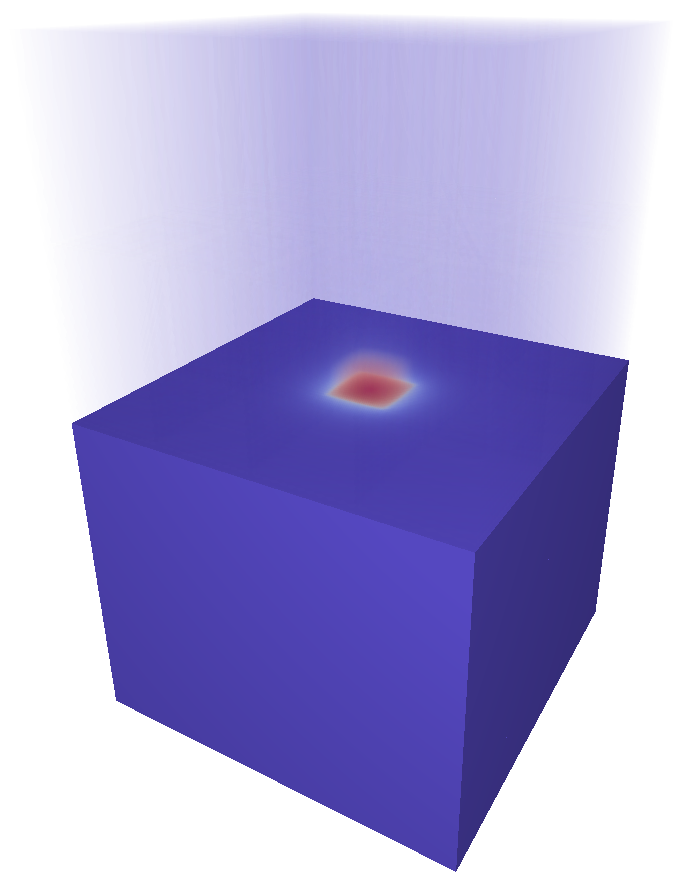
\includegraphics[width=3cm]{images/kripke}
	\caption{\label{kripke}Image produced using the operations described in Section~\ref{sec:results}.}
\end{figure}
\input{acks.inc}



\bibliographystyle{ACM-Reference-Format}
\bibliography{ISAV_Alpine} 

\end{document}
